\pattern{State}
\begin{summary}
    Given an object that needs to change its behaviour based on its
    internal state at run-time, the {\bf State} pattern encapsulates the number
    of states in a given context. A context calls its cooresponding
    state to perform specific behaviour, which changes based on the
    current value of the state object.

    This pattern should be used when the application's behaviours can be
    clearly divided into independent states that have specific and distinct
    behaviours, and when the application needs to be able to change its state
    and behaviours at run-time.

    Example. A flashlight has two states, on and off. When the flashlight is on,
    pressing the power button will turn off the flashlight, and vice versa.
\end{summary}

Implementation details: \begin{itemize}
    \item {\sc Context}: an instance of a class that owns (contains) the state.
        The context is an object that represents a class that can have more
        than one state.
    \item {\sc State}: an abstract class or interface. {\sc State} is the base
        class for all possible states. It defines all possible method
        signatures that all states must implement.
    \item {\sc ConcreteState}: a class that implements the actual state
        behavior for the context object. It inherits from the base {\sc State}
        class. The {\sc ConcreteState} class must implement all methods from
        the abstract base class {\sc State}.
\end{itemize}

The State design pattern allows full encapsulation of an unlimited number of
states of a context. The context object calls its state object to perform
specific behavior. The behavior is differentiated by the concrete state at the
run-time.

\comparison{\begin{itemize}
        \item Maintainability: Adding, removing, and modifying states is
            streamlined and simple via modifying the corresponding concrete
            state object.
        \item Readability: Improved cohesion due to aggregation of all
            behaviours of a given state in its corresponding concrete state
            class.
        \item Low coupling: Each state is independent of each other states'
            behaviour and modifications
    \end{itemize}

}{\begin{itemize}
        \item Maintainability: Since each concrete state is implemented as a
            class, more classes are required and more code needs to be written
        \item Maintainability: must implement all the functions in the abstract
            state, even if a given class is not related to a function used
            primarily in a different class.
        \item Maintainability: Difficult to maintain due to all states being
            required to implement a new function when new functionality is
            added to the interface. 
    \end{itemize}
} %END comparison

\begin{nfps}
\item[Scalability]: The State design pattern allows an unlimited number of
    states for a given object.
\item[Adaptability]: Adding, removing, and modifying states is as simple as
    modifying a concrete object class.
\item[Dependability]: Since each state is independent of the others, states
    with errors do not interfere with the functionality of other states.
\item[Negative Maintainability]: Since each state requires a separate class,
    there can be a large number of concrete classes, resulting in the code base
    being harder to maintain. In addition, since every method in the abstract
    class must be implemented in the concrete classes, much more code needs to
    be written.
\end{nfps}

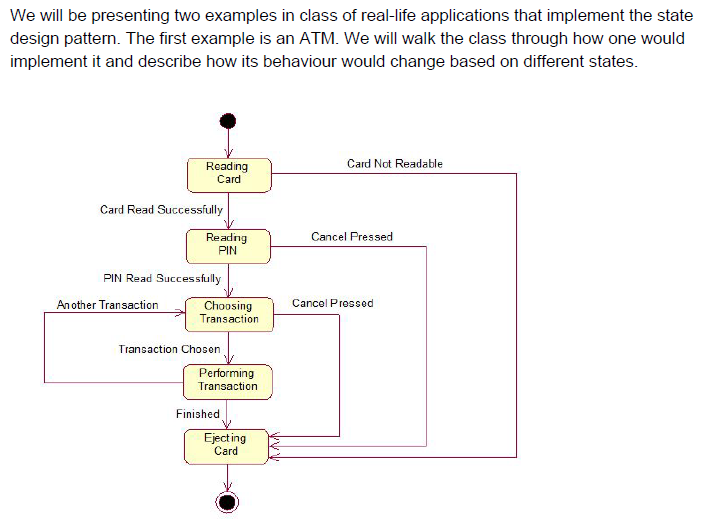
\includegraphics[width=0.5\textwidth]{./state1}
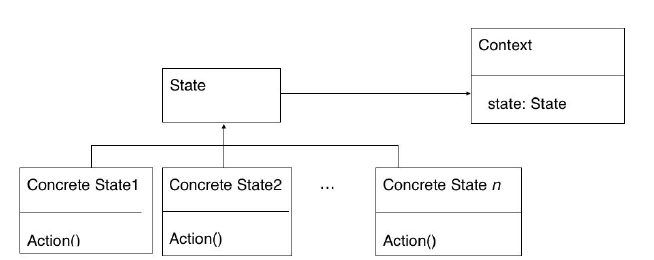
\includegraphics[width=0.5\textwidth]{./state2}

